\documentclass[../mathNotesPreamble]{subfiles}
\begin{document}
%\relsize{1.4}
  \section{JIT 5.1: Angles}
  
    \noindent
    \begin{minipage}[t]{0.6\linewidth}
      \begin{defn*}
        The \textbf{unit circle} is the circle of radius 1 that is centered at the origin.
      \end{defn*}
      \begin{defn*}
        The angle corresponding to an arc length of 1 on a unit circle is called a \textbf{radian}.
      \end{defn*}
    \end{minipage}%
    \begin{minipage}[t]{0.4\linewidth}\ 
     
      \begin{flushright}
        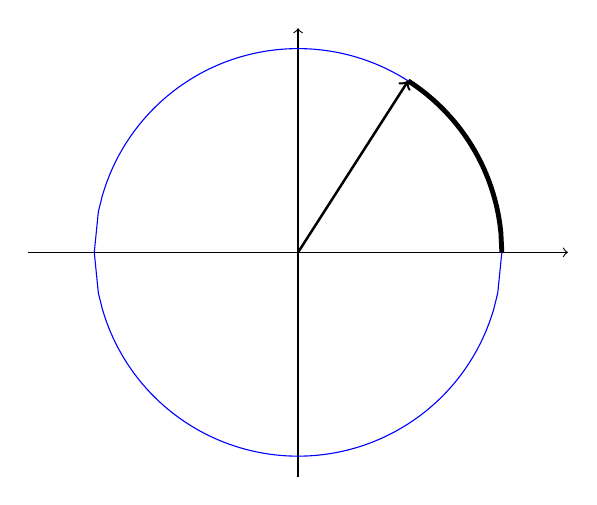
\begin{tikzpicture}[scale=1.0]
          \begin{axis}[
            axis lines=center,
            axis equal, 
            axis line style={->},
            xmin=-1.1, xmax=1.1,
            ymin=-1.1, ymax=1.1,
            xmajorticks=false,
            ymajorticks=false,
            ]
              \addplot[domain=-1:1, blue, samples=101] {sqrt(1-x^2)};
              \addplot[domain=0.5403:1, black, samples=101, line width=1.75pt] {sqrt(1-x^2)};
              \draw[->, black, line width = 0.9pt] (axis cs:0,0)--(axis cs:0.5403,0.84147);
              \addplot[domain=-1:1, blue, samples=101] {-sqrt(1-x^2)};
          \end{axis}
        \end{tikzpicture}
      \end{flushright}
    \end{minipage}
    
    A circle is $2\pi$ radians or $360^\circ$. Thus:
      $$2\pi=360^\circ \Longrightarrow 1=\dfrac{180^\circ}{\pi}=\dfrac{\pi}{180^\circ}$$
    \vspace*{\stretch{1}}

    \pagebreak
\end{document}
